\section{Problems and Solutions}
\markright{Problems and Solutions}

This section contains two simple Java programs that introduce the language and basic programming logic. The first program demonstrates the basic syntax and the execution flow of a Java class, while the second program applies the concept of looping and conditional checking to solve a practical numerical problem.

\subsection{Problem 1: Hello World Program}
This program writes a basic message to the console using Java's standard output method. It is commonly used as the first step in learning any programming language because it demonstrates the required class structure, method definition, and program execution process. The program confirms that Java is installed correctly and that the development environment is ready for coding.

\subsubsection{Code}
\begin{lstlisting}[language=Java, caption={}, numbers=left]
package lab05;

public class HelloWorld {
  public static void main(String[] args) {
    System.out.println("Hello, World!");
  }
}
\end{lstlisting}

\subsubsection{Output}
\begin{figure}[H]
  \centering
  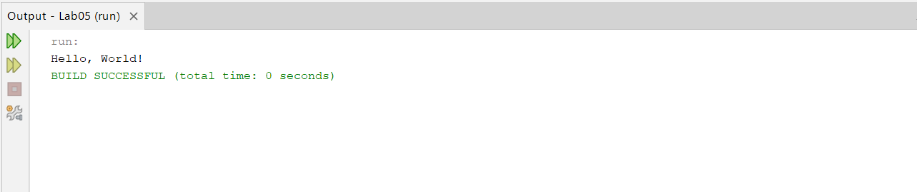
\includegraphics[width=0.8\textwidth]{lab-05/assets/output1.png}
  \caption{Output of the Hello World program showing successful Java execution.}
\end{figure}

\subsection{Problem 2: Prime Number Checker}
This program reads an integer from the user and determines whether it is a prime number. The algorithm uses a loop to test divisibility from 2 up to the square root of the number and uses a conditional statement to decide if the value is prime or composite. This example illustrates how repetition and decision-making are combined to solve a common computational task.

\subsubsection{Code}
\begin{lstlisting}[language=Java, caption={ }, numbers=left]
package lab05;

import java.util.Scanner;

public class FindPrime {
  public static void main(String args[]) {
    Scanner input = new Scanner(System.in);
    boolean isPrime;

    System.out.print("Enter a number: ");
    int num = input.nextInt();

    isPrime = num >= 2;

    for(int i=2; i <= num/i; i++) {
      if((num % i) == 0) {
        isPrime = false;
        break;
      }
    }

    if(isPrime) System.out.println("Prime");
    else System.out.println("Not Prime");
  }
}
\end{lstlisting}

\subsubsection{Output}
\begin{figure}[H]
  \centering
  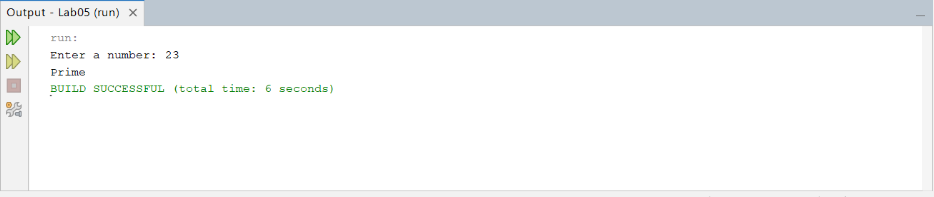
\includegraphics[width=0.8\textwidth]{lab-05/assets/output2.png}
  \caption{Output of the prime number checking program for a sample input value.}
\end{figure}
